\documentclass[../../main.tex]{subfiles}
\begin{document}

This section will provide a description of the elements of the given pan-tilt system as well as an analysis of possible approaches to satisfy the problem description described in section \ref{sec:ProblemDescription}.

\subsection{Description of Physical Setup}
The pan-tilt system is made of aluminium extrusions and can be divided into two sections, a stationary lower section and a upper movable section. The movable section consists of two \textit{frames}, the pan frame and the tilt frame. The tilt frame is a simple square, and the pan frame is u-shaped with the tilt frame attached inside as illustrated on figure \ref{fig:Pan_Tilt_Drawing}.

From initial experiments with the pan-tilt system it is found that significant friction is present in joints and bearings. It is also found that the friction varies according to the position of the frame. Probably these irregularities stem from the physical setup being poorly constructed, as it is visibly skewed.  

Each frame is actuated by a DC motor equipped with an incremental encoder \cite{}. The resolution of the encoders is 360 counts per revolution of the output shaft. The encoders make it possible to determine an offset from the initial position. Hall effect sensors \cite{} provide an index signal for each frame. The index signals are used to provide a reference point for the incremental encoders. From the change in position relative to the time, the velocity of the motor can be calculated. Both motors are connected to an H-bridge, which can be enabled with a PWM-signal to control the voltage over the motors. Furthermore the H-bridge also makes is possible to change the polarity of the voltage supplied, yielding a change in the motors turning direction.

\subsection{Controller Design}
The problem description states that a position controller has to be designed, however such a controller can take on many forms, leading to different design approaches and methods. Generally speaking, controller design can be divided into two categories, classical control which operates in the frequency domain and classical control which operates in the time domain. Both approaches will be examined in this section. First, however, some general crucial control theory concepts will be explored.
When designing a 

%Plant 
%Controller
Some important concepts in control theory is plant, which is a relation between an input signal and an output signal.  
Two important concepts from control theory are open loop and closed loop. The difference between them is that in a closed loop system there is feedback from the output of the system to the input, while in an open loop system there is no feedback. This is also illustrated on figure \ref{fig:Open_Close_loop}.


When it comes to controller design two methods, which are appropiate for
\textit{Controll oer} design can be divided into two methods, classical control and modern control. Different methods of designing the controllers are present such as \textit{PID controllers} and state feedback, while other methods exist, it is beyond the scope of this project to discuss those. The methods and techniques associated with those will be described further below. Two concepts are introduced working with control theory namely open loop and closed loop illustrated on figure  The difference in the concepts are the feedback in closed loop, while there is none in open loop.

% introduktion til kontrol, keywords: open loop, closed loop, etc. 

\subsubsection*{Single controller vs. cascaded controllers}

\subsubsection*{Classic Control theory}

\subsubsection*{Modern Control theory}

% The pan and tilt motor controlling the pan-tilt, is 12V motors fully equipped with encoders and can be controlled with a PWM signal. By using the two H-bridge it is possible change the polarity of the voltage applied to the motors and there by change the direction. 
% The encoders transmits signals when ever the position of the motors changes, thus it can be used to determined the angular position relative to the initial position and the rate of change. 
% \begin{figure}
%     \centering
%     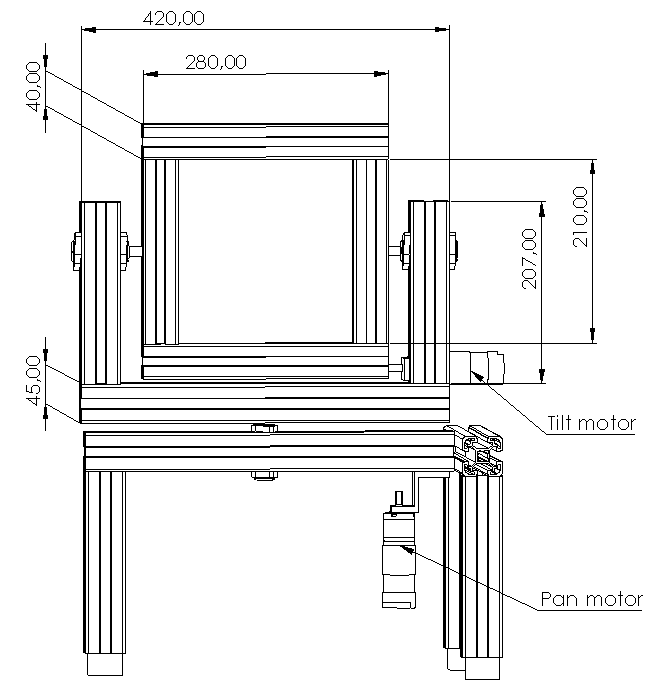
\includegraphics[width=0.7\textwidth]{Sections/Miscellaneous/Images/PhysicalMotorModel.png}
%     \caption{Drawing of the pan-tilt system with physical measures in \SI{}{\milli \meter}.}
%     \label{fig:Pan_Tilt_Drawing}
% \end{figure}

%As mentioned in section \ref{sec:ProblemDescription}, the physical setup introduces friction and limitations to the system from joints, bearings and the motors. % The non-linear friction of the system is difficult to model. The friction makes the system unpredictable in relation to the modelled system, thus it is difficult to make any assumptions and make conclusions regarding the system. 
%The limitations such as the velocity of the motor or the pan frame's limited range of motion will effect the dynamics of the system. The limitations can be taken into account by implementing \textit{saturation} on the control signal, and the velocity in the simulation.

% When the control signal goes beyond the saturation limits will keep winding up yielding a bigger difference between the wanted control signal and the saturated control signal. This means the control signal will take longer to return to the unsaturated area. To counteract this behaviour anti-windup can be added to the controller. Multiple methods for implementing anti-windup exists, only the methods back-calculation and conditional integral will be examined. Conditional integral is the simplest method, where the integral term is only evaluated when the control signals not is in beyond the saturation limits. The principle behind the back-calculation method is to subtracting the unsaturated signal from the saturated, and the adding a fraction of the difference to the integral input.  

% can be taken into account by implementing saturation in the modelling of controller and plant.
%Different approaches to anti-windup is available and is often related to the controller in question.

% When controlling the pan-tilt system a user-input is required with a position for the motors. When 
As a voltage is applied across a motor, a current will run through the coils of the motor, while the motor will start spinning with an angular velocity. Current and velocity are two aspects of the motors that change at a higher rate than the position of the motor, while also influencing the position of the motor. 

Using a single \textit{controller} it is not a problem as long as the relation between the current and position remains the same. 
However if any noise is introduced to the system altering the relation between the current and position, the response of the position controller is retarded. This is due to the current changing rapidly compared to the position. 

Adding a controller dealing with the velocity and current and implementing the controllers in cascade, the outer controller is isolated from the faster changes of velocity and current, leaving the designated controllers to control them. When implementing the controllers in cascades, the position controller feeds the velocity controller with the velocity reference point and the velocity controller feeds the current controller, which results in the required current for the motor to achieve the desired position. This means that the velocity and current controller will deal with any noise such as friction, thus achieving a faster compensation to noise and a faster response overall. However this introduces three controllers, which have to be tuned individually, making the intuitive process of tuning more challenging \cite{CascadeControl}.
%Anti windup

\begin{figure}[H]
    \centering
    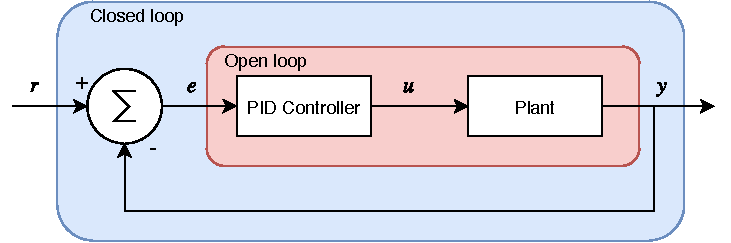
\includegraphics[width=0.7\textwidth]{Sections/Miscellaneous/Images/Open_closed_Diagram.pdf}
    \caption{Figure illustrating the concept of open and closed loop. }
    \label{fig:Open_Close_loop}
\end{figure}





\subsection*{Classical Control Methods}
A traditional method for designing a controller for a motor is to use a PID controller. Though many controller configurations using parts of the PID controllers design exists, only the full PID controller will be examined. The block diagram of a PID controller can be seen on figure \ref{fig:PID_controller}. As seen on the block diagram
a PID controller utilises a feedback loop. The feedback is subtracted from the reference signal resulting in an error, which then is send to the controller. The controller consist of three terms: a proportional term, an integral term and a derivative term. Each evaluated separately and then combined to yield the output of the controller. If only the proportional term is used, a steady state error between the output and the reference will always be present. Therefore the integral term is introduced to eliminate the steady state error, as the integral will keep increasing until there is no steady state error. The derivative term is used to control the overshoot of the step response.

Another way to correct steady state error is feedforward. Feedforward
\begin{figure}[]
    \centering
    \includegraphics[width=0.7\textwidth]{Sections/Miscellaneous/Images/PID-control-diagram.png}
    \caption{Block diagram of a PID controller with an additional feedforward implemented.}
    \label{fig:PID_controller}
\end{figure}

% The proportional term is proportional to the error, but leaving the output with a steady state error, due to the term always requiring an error to function. To correct this steady state error, feedforward can be introduced, where the proportional signal is added as seen on equation \ref{eq:feedforward}, where $G$ is the transfer function of plant and $r$ is the setpoint.
% \begin{equation}\label{eq:feedforward}
%     u_{ff}=\frac{1}{G(0)}r(t)
% \end{equation}
% However feedforward is sensitive to modelling uncertainties, due to it heavily relying on the design of the plant. Instead the integral term can be implemented, integrating the error thus eliminating the steady state error. To increase the settling time of the controller the derivative term can be added, which is an anticipatory term looking at the trend of the error, thus making it possible to change the direction of the signal, if overshoot or oscillating tendencies occurs. However the derivative term is vastly sensitive to noise, making it necessary to filter the signal upon implementation of the controller. 

To achieve the desired response of the system, the different gains of the PID controller must be found. Finding the gains for the PID controller different methods are available each with different advantages. A method is pole placement, where the location of poles in the closed-loop system is analysed. This introduces the prerequisite, that the system must be known. If a model of the plant is not available other means for tuning is present. A method is the Ziegler-Nichols method, where the controller is tuned by examining the input and output of the system. By examining a step response of the actual system it is possible to deduct the \textit{lag} of the system, the amplitude and the rise time of a first order system. From these parameters its is possible to make an estimation for the gains of the PID controller.

Having a transfer function of a given plant, $G(s,K)$, with an unknown parameter K, it is possible to describe the movement of the poles in the s-plane using the root locus method. By looking at the rise time, overshoot and settling time it is possible to estimate where in the s-plane the poles can be placed to ensure the desired behavior of the system. %Limitations for the placement of the poles can be found. 
With the root locus method, it is possible to tweak the controller in such a manner, that the system satisfies the requirements.

Having a system in saturation the integral term will continue to increment in order to reduce the error. However this is not a desired behavior, creating a slower response of the control signal, $v$, goes below saturation. Figure \ref{fig:anti-windup} illustrates the implementation of back calculation for a PID controller. When the system is in saturation, and therefor not able to increase, the control signal $u$ is constant. The time tracking constant, $\frac{1}{T_t}$ determines how quick the integrator is changed. When implementing anti-windup it can be executed using back-calculation or conditional integration. Back calculation works by subtracting the saturated signal, $u$, with $v$, thus when the system is saturated, the signal $e_s$ is negative. This means that a value is subtracted from the integral term in the controller resulting in a lower value of $v$. This decreases $v$ until the point when $v=u$ and $e_s$ is zero. Conditional integration works by simply keeping the integration term constant in the controller once saturation is reached. 

\begin{figure}
    \centering
    \includegraphics[width=0.7\textwidth]{Sections/Miscellaneous/Images/PID-Anti-windup-BackCalc.png}
    \caption{Diagram of anti-windup using back calculation. $T_t$ is the tracking time constant and $e_s$ is the saturation error.}
    \label{fig:anti-windup}
\end{figure}

\subsection*{Modern Control Methods}
Modern control methods introduces the use of state feedback. The general idea is to achieve the correct steady state response to a command signal. This is done by tweaking a gain on the state feedback, such that the general state space model yields equation \ref{eq:gen_statespace}. To function correctly a prerequisite is that the model is an exact replica of the actual system, which can be difficult to achieve.
\begin{equation}\label{eq:gen_statespace}
    \begin{split}
        \Dot{x}&=Ax+Bu \\
        y&=Cx \\
        u&=Fx
    \end{split}
\end{equation}
where $A$ is the system matrix, $B$ is the input matrix, $x$ is the state, $u$ is the control signal, $y$ is the output and $C$ is the output matrix. $F$ is the state feedback matrix. 

\begin{figure}
    \centering
    \includegraphics[width=0.8\textwidth]{Sections/Miscellaneous/Images/Integral_Observer_Anti_windup.png}
    \caption{Block diagram of an integral controller with observer and anti-windup.}
    \label{fig:Integral_Observer_Diagram}
\end{figure}

An approach of controlling the system using state feedback, without the need to have an exact model, is integral control as seen on figure \ref{fig:Integral_Observer_Diagram}. The integral feedback provides zero steady state error by integrating the error. Taking basis in the state space form equation \ref{eq:gen_statespace} and adding an additional feedback, the input is given as described in equation \ref{eq:input_integral}.
\begin{equation}\label{eq:input_integral}
    u(t)=Fx(t)+F_Ix_I(t)=
    \begin{bmatrix}
        F & F_I
    \end{bmatrix}
    \begin{bmatrix}
        x\\
        x_I
    \end{bmatrix}
\end{equation}
where $F$ is the state feedback matrix, $F_I$ is the integral matrix and $x_I(t)$ is given by:
\begin{equation}
    \begin{split}
        x_I(t)=\int_0^t y(\tau)-r(\tau)\,d\tau
    \end{split}
\end{equation}
where $t$ is the time, $y$ is the output and $r$ is the reference. However this introduces more variables to tune, and requires that every state is known. Means to estimate states of a given system is available. The estimation can be achieved by introducing an observer to the system, which is illustrated on figure \ref{fig:Integral_Observer_Diagram}. The observer aims to mirror the plant and by that making it possible to estimate a given state. The observer introduces an observer gain, $L$, which is proportional with the difference between the output from the plant and the estimated observer output. The observer state space model is as seen in equation \ref{eq:Obs_state_space}, where $L$ is the observer gain and $\hat{x}$ is the estimated state and $\hat{y}$ is the estimated output.
\begin{equation}\label{eq:Obs_state_space}
    \begin{split}
        \Dot{\hat{x}}&=A\hat{x}+Bu+L(C\hat{x}-y)\\
        \hat{y}&=C\hat{x}
    \end{split}
\end{equation}
The observer gain is found by equation \ref{eq:observer_error} and to insure that the system is stable the eigenvalues should be placed in the left open half plane.
\begin{equation}\label{eq:observer_error}
    \Dot{e}=(A+LC)e
\end{equation}
where $e=\hat{x}-x$. However a prerequisite using the observer is making sure, that the system is observable. An observer cannot be implemented, if the system is unobservable. Another challenge using the observer is tuning the observer gain and generally estimating the plant. 

To take in to account that there are psychical limitation in form of saturation an anti-windup in form of the gain M on figure \ref{fig:Integral_Observer_Diagram} can be added. The anti-wind looks at the difference between the control signal with and without saturation and if there is a different it prevent the integral term to windup. 
If saturation happen the dynamic of the observer controller changes to:
\begin{equation}\label{eq:anti-windup_state_space}
    \begin{split}
        \Dot{\hat{x}}&=A\hat{x}+LC\hat{x}+MF\hat{x}\\
        \hat{y}&=C\hat{x}
    \end{split}
\end{equation}

The LQR (Linear Quadratic Regulator) is method concerned with minimising the cost of operating a linear system. The LQR is an algorithm trying to find the optimal state feedback controller. The control of a system is said to be optimal, if it minimizes the cost function.
\subsection*{Modelling}
%modelling, continuous vs discrete
Upon modelling and simulating the controllers and the system, it is important to keep in mind that an actual implementation of a controller is discrete rather than continuous. This can be done by directly designing the controller in discrete time. Another approach is designing a continuous controller and then approximating it in discrete time.

A method to implement the controller is the Tustin's method, which dictates a certain way of describing the parameter for the controller. Equation \ref{eq:continuous_Vs_discrete} illustrates a continuous PID controller versus a discrete PID controller designed using the Tustin's method.
\begin{equation}\label{eq:continuous_Vs_discrete}
    \begin{split}
        u(s)&=\left(k_P+\frac{k_I}{s}+k_Ds\right)e(s)\\
        u(kT+T)=k_Pe(kT+T)+u_1(kT)+&k_I\frac{T}{2}(e(kT+T)+e(kT))+k_D\frac{2}{T}(e(kT+T)-e(kT))-u_D(kT)
    \end{split}
\end{equation}
where $u(s)$ is the control signal in continuous time and $u(kT+T)$ is the control signal in discrete time. $T$ is the sampling time, $e$ is the error and $k_p$, $k_I$ and $k_D$ are the PID gains. As seen from equation \ref{eq:continuous_Vs_discrete} the terms depend on the sampling time, thus it needs to be known. The sampling frequency for a discrete controller should be approximately 20 times larger than the closed-loop bandwidth of the system otherwise special care needs to be taken when designing the controller, which will not be discussed further. 

\subsection*{Micro Controller}
Implementing at least two controllers on the same micro controller and having to accommodate other tasks such as SPI and UART in parallel. It would be advantageously to implement some sort of scheduling algorithm. The easiest way of implementing a scheduling algorithm is by the use of an operating system (OS). Various types of operating systems exist, though in this project only two operating systems has been evaluated, Run To Complete Scheduler (RTCS) and FreeRTOS. The RTCS uses a cooperative scheduling algorithm, where the task voluntarily has to give up the CPU. This method provides a light weight overhead, though the risk of a task blocking the CPU is greater as no central allocation of resources exists. % The run to complete scheduler (RTCS) constitutes such an algorithm and is based on a cooperative scheduling where a running task wont be interrupted by other tasks, unless the task voluntarily yield control. Thus to achieve a seemingly multitasking system all tasks must cooperate to prevent starvation of tasks. 
The FreeRTOS uses preemptive scheduling algorithm where a central master is responsible for the allocation of resources. The central master can preempt a task whenever it is wanted, therefore minimizing the probability of starvation occurring.

% could also be implemented, which opposed to the RTCS allow the scheduler to preempt tasks when the allocated CPU time of the task is used. Switching between tasks does however introduce overhead.\\

% Ideally controllers implemented on the micro controller would need and use new data as soon as it is sampled. Intertask communication also demands management of datasharing, since it is usually unsafe for two tasks to access the same specific data. To have the system use a scheduling algorithm and ensure reliable performance, an operating system (OS) can be used. The real-time operating system (RTOS) is an OS using preemptive scheduling and is intended to have tasks process data as it comes in. It also allows for prioritization of tasks, so timing of more time-critical tasks does not become compromised. 



%Another algorithm is FreeRTOS, which schedules tasks based on priority and CPU time and constitutes a real time operating system (RTOS). In addition FreeRTOS also provide a broad range of predefined functionality regarding queues and semaphores.  


\end{document}